%How did Google Glass come about? History!
%Mobiles today are used as a nervous tick. It is a distraction and something that pulls your attention away from the real world. At least that is what Sergey Brin, one of the founders of Google, claimed during a Ted Talk presentation in February 2013.\cite{tedtalkWhyGlass} Brin stated that if he was a smoker he would probably light a cigarette at those times when he now uses his phone.
%\url{http://www.ted.com/talks/sergey_brin_why_google_glass}

%Brin and his team wanted to create something that would make interaction with technology easy and fast and not distract from reality. They wanted to keep the information more handy and close by than a phone stuck in the users pocket. But they also wanted to keep the line of sight free. Thad Starner, technical lead/manager on Google Glass, wrote in an article in 2013,\cite{6504855} that he sought out to build something as intuitive as a watch. An extension of the self, as he stated. And so Google started working on Project Glass. 




% The idea behind Glass was to minimise the time between intention and action
% users should not have to bring up something from their pockets each time they want to interact with technology
% they should be able to just simply interact
% They wanted to create something as intuitive as a watch. 
% checking the watch is something a user might do without actually thinking about what the time is.
% they might have to check again if someone were to ask them what the time is.
% Glass should be an extension of the self rather than another device.
% // Thad Starner - technical lead/manager on Google Glass

% Sergey Brin, one of the founders at Google, has similar ideas
% ted talk he spoke about how checking the phone was something he did without reason
% putting notifications more easily accessible would minimise interaction with technology because the user
% would not have to check if any updates have come in, they would know right away



On April 4th, 2012, Google announced ``Project Glass''.\cite{GoogleGlassConcept} Google Glass, as the device is now known, was under development for several years at Google's research and development department, Google X. As part of teh announcement Google stated:  ``We think technology should work for you---to be there when you need it and get out of your way when you don’t.''\cite{GoogleGlassAnnouncement} Serge Brin, one of the founders of Google, did a Ted Talk in February 2013\cite{tedtalkWhyGlass} where he talked about why they decided to produce the device. His argument was that users stayed on their smartphones for too long. Bring also argued that when users were using their smartphones they were looking down on a screen and were not aware of their surroundings. Instead Google wanted to create a device that would give the user notifications that could quickly be dealt and done with.\\

Thad Starner, technical lead/manager on Google Glass, claimed that Google Glass is supposed to be an extension of the self.\cite{6504855} He compared Google Glass to a watch. A watch is easy to access and the access is also instant. Starner said that with Google Glass, Google wanted to minimise the time between intention and action. 


\subsection{What is Google Glass?}
\label{subsec:googleglass}
Google Glass, or simply Glass as the device is known within Google, is a head mounted display (HMD) that can be seen as an augmented reality device\footnote{See section \ref{subsubsec:augmentedrealityvsvirtualreality}} designed to bring notifications to the user more easily than a smartphone does. According to Google ``Glass is designed to be there when the user needs it and to stay out of the way when the user does not''.\cite{glassDesignPrinciples} Google Glass is meant to give the user relevant information at relevant times.\\ 
%\url{https://developers.google.com/glass/design/principles}

Google Glass is partially controlled via a touchpad (it can also be controlled with voice command). The touchpad sits on the right hand side of the user's glass frame and runs from the temple to the ear. When the user touches anywhere on the touchpad Google Glass ``wakes up'' from stand by and displays the start screen (which consists of a clock). The display is mounted above the user's line of sight, on the right hand side. The display can be slightly adjusted so that the user can see everything displayed. \\







	\begin{figure}[ht!]
		\centering
		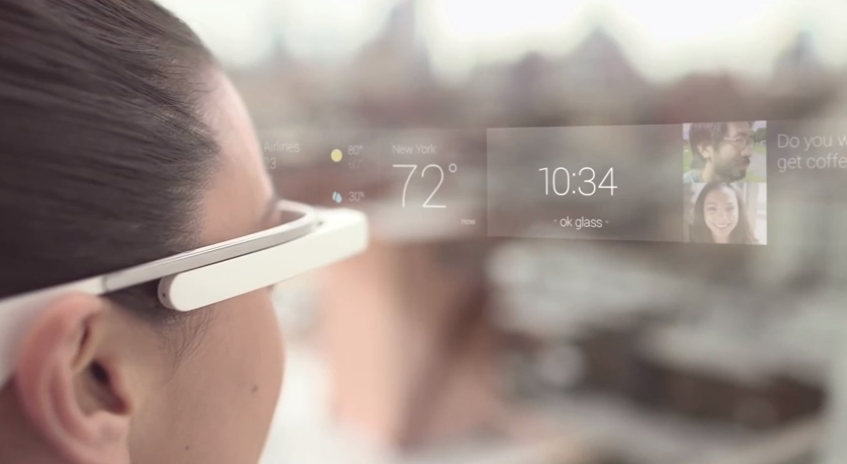
\includegraphics[width=110mm]{images/GoogleGlassUI}
		\caption{A virtual representation of the Google Glass user interface as the graphical user interface is perceived by the user.\cite{ImagesGoogleGlassUI}}
		\label{GoogleGlassUI}
	\end{figure}
	
	
	




The graphical user interface (GUI) is called a timeline (see Figure \ref{GoogleGlassUI}). The timeline consists of a row of cards. Cards are basic applications such as a clock or information about the weather. Cards can also represent more in-depth applications, on Google Glass called ``Immersions''. An immersion handles activities such as browsing an image gallery or playing a game.\\

On the timeline cards to the left of the home screen are upcoming activities such as an event in the user's calendar or an upcoming flight. Cards to the right of the home screen are from the past. Cards from the past will for instance show text messages or photos. When the user wants to turn of Google Glass the user swipes down on the touchpad. Swiping down on the touchpad will put Google Glass in stand by. If the user wants to turn of Google Glass entirely there is a power button on the opposite side of the touchpad. Holding down the power button for a few seconds will turn of Google Glass. For a better visual understanding of how Google Glass works see Figure \ref{GoogleGlassUI} as well as the video referenced in the caption.\\

%Glass uses a small display placed to the upper right of the user's line of sight and is mounted on the user as a regular pair of glasses. Equipped with a camera, microphone and speakers it is capable of performing a lot of the tasks users normally would do on a smartphone such as taking photographs, video chatting, writing text messages.

The principles behind designing for glass is to keep the information relevant. Google ranks different computational devices and services in terms of time periods. Google talks about how the cloud stores information ``forever'', a computer keeps about a years worth of information, a mobile phone is keeping track of the last month and Glass are for the present.

Therefore Google asks developers to keep the information relevant and simple. Glass is designed not to get in the way of the user and, as stated previously, be usable when the users wants to.\cite{glassDesignPrinciples}
%\url{https://developers.google.com/glass/design/principles}

\subsubsection{Augmented Reality vs Virtual Reality}
\label{subsubsec:augmentedrealityvsvirtualreality}

[TODO WRITE ABOUT HUD AND HMD]

When discussing head mounted displays it is possible that the first image that pops into ones head is similar to Figure \ref{OculusRift}. What is important to note about Oculus Rift (Figure \ref{OculusRift}) and other similar product that completely covers the user's eyes is that these are all virtual reality devices. Virtual reality is not the same as augmented reality, which is what Google Glass gives the user.



	\begin{figure}[ht!]
		\centering
		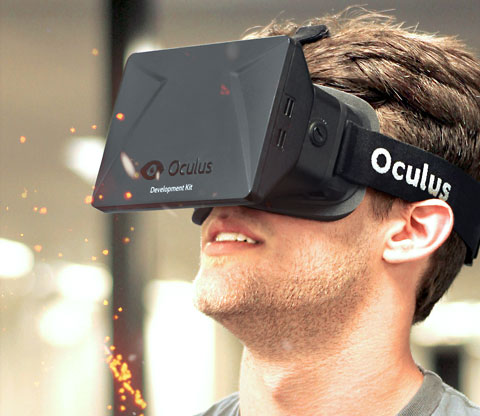
\includegraphics[width=110mm]{images/OculusRift}
		\caption{The virtual reality device Oculus Rift is a head mounted display that covers the user's eyes completely\cite{ImagesOculusRift}}
		\label{OculusRift}
	\end{figure}





The difference lies in how much of what the user can see is computer generated. In a virtual reality the entire environment is computer generated. Augmented reality on the other hand is based in reality where computer generated elements of the environment help enhance reality. In other words: virtual reality replaces reality and augmented reality enhance reality. Since Google Glass does not remove the user from reality but rather display information that can be consumed at the same time as the user experience the real world Google Glass is an augmented reality device compared to Oculus Rift which is a virtual reality device.

TODO --- ADD HUD vs AUGMENTED REALITY!!!!!!


%What is it?
%Augmented Reality vs Virtual Reality
%Define Augmented Reality
%Define Virtual Reality


\subsection{User Interface}
\label{subsec:userinterface}
The Google Glass graphical user interface (GUI) is called a timeline~\cite{ImagesGoogleGlassUI} (see Figure~\ref{GoogleGlassUI}). The timeline consists of a row of cards. Cards are basic applications such as a clock (see Figure~\ref{GoogleGlassCards}~(a)) or information about the weather. Cards can also represent more in-depth applications, on Google Glass called ``Immersions'' (see Figure~\ref{GoogleGlassCards}~(b) and~(c)). Immersions handle activities such as browsing an image gallery or playing a game.

	\begin{figure}[ht!]
		\centering
		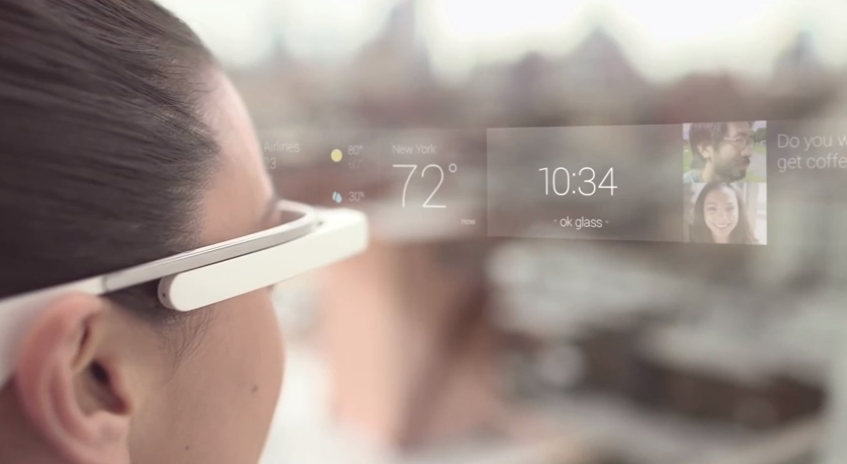
\includegraphics[width=110mm]{images/GoogleGlassUI}
		\caption{A visualisation of the timeline as the timeline is perceived by the user~\cite{ImagesGoogleGlassUI}.}
		\label{GoogleGlassUI}
	\end{figure}

The first screen the user sees when starting up Google Glass is the home screen. The home screen displays a clock and also shows the text "ok glass", as seen in Figure~\ref{GoogleGlassCards}~(a). The home screen is a part of the timeline and acts as the center point. Cards to the left of the home screen are upcoming activities such as an event in the user's calendar or an upcoming flight. Cards to the right of the home screen are from the past. Cards from the past will for instance show text messages or photos.

	\begin{figure}[ht!]
		\centering
   	\subfloat[The Google Glass home screen is a card that displays a clock.]{{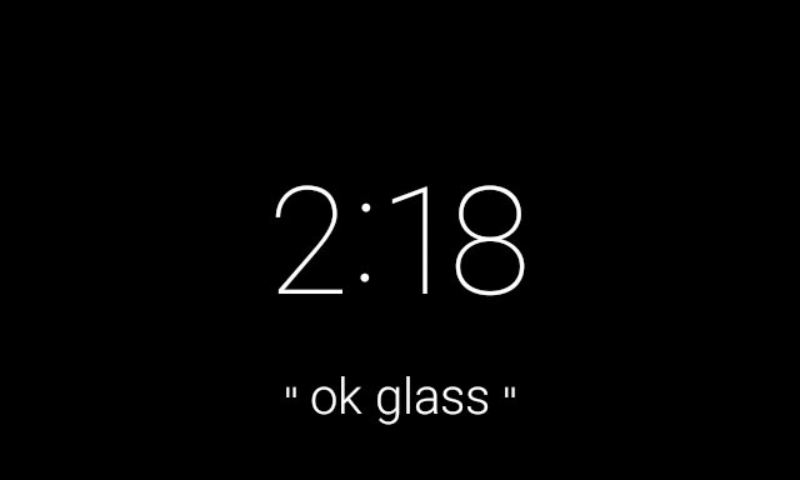
\includegraphics[width=70mm]{images/GoogleGlassHomescreen} }}
  	 \qquad
   	\subfloat[The card ``Explore stars'' represents an immersion.]{{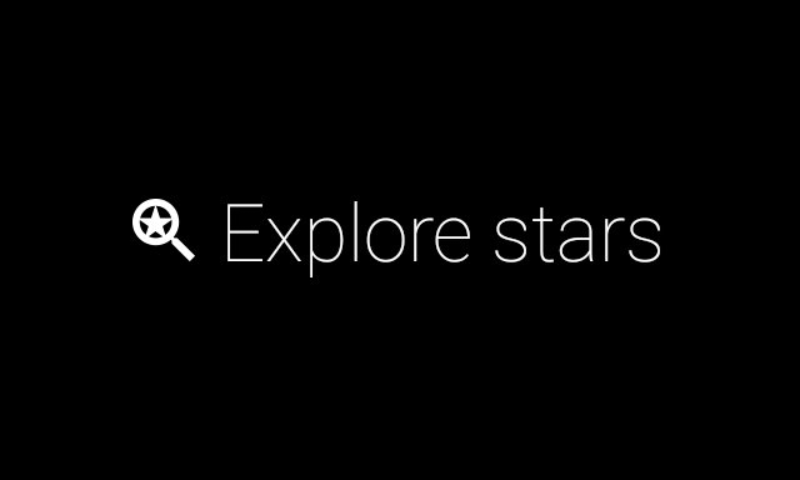
\includegraphics[width=70mm]{images/GoogleGlassStarImmersion} }}
   	\qquad
	\subfloat[The immersion ``Explore stars'' allows the user to look around at stars using the built-in head motion tracker.]{{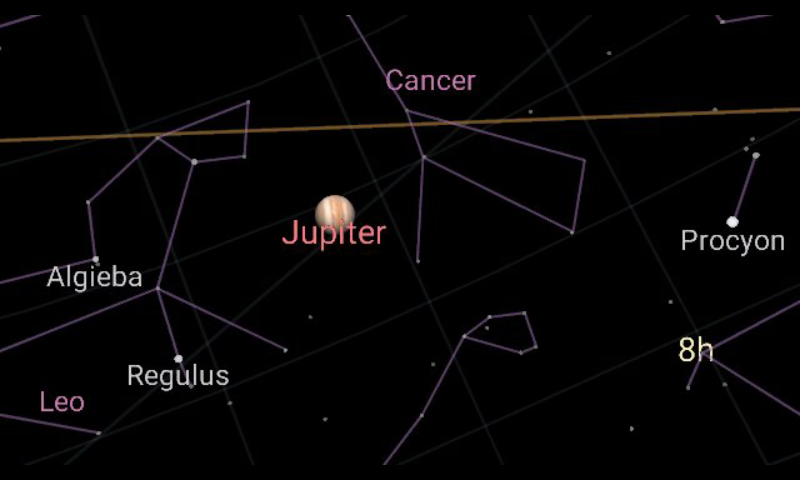
\includegraphics[width=70mm]{images/GoogleGlassStarImmersion2} }}
   	\qquad
		\caption{Cards can either display basic applications or represent immersions.}
		\label{GoogleGlassCards}
	\end{figure}

In order to move left on the timeline (forward in time) the user must swipe a finger backwards on the touchpad. In order to move right on the timeline (backward in time) the user must swipe a finger forward on the touchpad. The fact that the user must swipe backwards when stepping forward in time might not seem especially intuitive. In western culture a timeline is normally represented as going from left to right. One example is books, where the reader not only reads each line from left to right, but also turn pages from the right (the future) to the left (the past). However, on Google Glass, the swiping action could be thought of as swiping cards behind the back. Swiping forward when stepping backwards in time would then in turn mean bringing cards placed behind the back into focus. Cards in the past are behind the user while cards in the future are in front of the user.

When the user wants to turn off Google Glass the user swipes down on the touchpad. Swiping down on the touchpad will put Google Glass in stand-by mode. If the user wants to turn off Google Glass entirely, in other words power down the device, there is a power button on the opposite side of the touchpad. Holding down the power button for a few seconds will turn off Google Glass. For a better visual understanding of how Google Glass works see Figure~\ref{GoogleGlassUI} as well as the video referenced in the caption.

Google Glass uses a Bone Conduction Transducer (BCT) to transfer sound to the user~\cite{GlassSpecs}. The BCT transfers sound to the inner ear by conducting sound through the bones of the skull~\cite{boneConductionWiki}. The advantage of this technique is that the sound maintains clarity, even in noisy environments. Also, since the user does not plug any earphone into their ears, external sound is not blocked out.

Google Glass also features a 5 megapixels camera~\cite{GlassSpecs}. The camera sits between the touchpad and the display, as seen in Figure~\ref{GoogleGlassHardware}~(b), and is capable of capturing video at a 720p resolution. The camera can be used for video conferencing, as Google showed in 2012~\cite{glassLiveDemo}, but the camera can for instance also be used when the user wants to scan a QR Code (see Section~\ref{subsec:qrcode}).

The user can also interact with Google Glass using voice commands. As seen in Figure~\ref{GoogleGlassCards} the home screen consists not only of a clock but also of the words ``ok glass'', in quotes. ``ok glass'' indicates to the user that voice commands are available. The voice command menu is accessed as soon as the user says the words ``ok glass''. Doing so brings up a list of voice commands available, as seen in Figure~\ref{voiceCommandMenu}.

	\begin{figure}[H]%ht!]
		\centering
		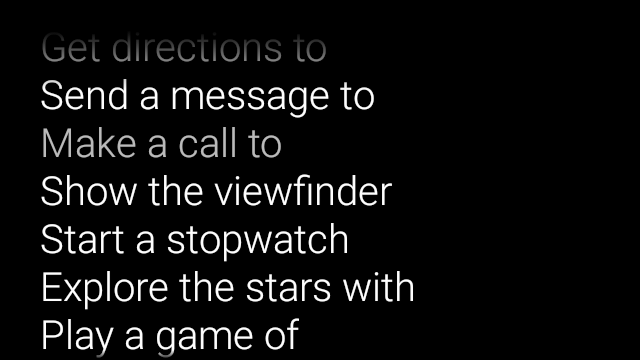
\includegraphics[width=110mm]{images/glassVoiceMenu}
		\caption{Saying ``ok glass'' will bring up the voice command menu~\cite{googleGlassVoiceCommand}.}
		\label{voiceCommandMenu}
	\end{figure}

In order to progress further the user must say one of the options being displayed out loud. Doing so will either make Google Glass perform the task spoken or give the user the option to add an input option to the task chosen. For instance, if the user where to say ``ok glass, Start a stopwatch'', Google Glass would start a stopwatch.

Google Glass also supports head motions as a form of input from the user. Head motions are not enabled in the timeline as a way of input but tilting the head may wake up Google Glass from stand by mode, if the user has enabled the head wake up feature~\cite{headWakeUp}. The head motion interface may also be used in certain immersions, such as ``Explore stars'' seen in Figure~\ref{GoogleGlassCards}~(c).
%The main way for a user to give input to Google Glass is via the touchpanel that is mounted on the right hand side of Glass, along the frame. Users are able to swipe as well as tap, which gives them control similar to that of a Smart TV's user interface. Where with a TV controller the user would maneuver with a simple cross layout (up, down, right and left) the buttons have on Glass been replaced by a touchpanel.\\

% Insert image of Google Glass graphical user interface here!!!

%The graphical interface is displayed at the top right through a projection coming from the right on a thick piece of glass. This technique lines up the image with the users sight but does not give any projection outwards.\\

%The interface is built with cards. Each card represents an activity.\\

%What’s unique?
%Standards?
%\url{https://developers.google.com/glass/design/}

\subsection{Compared to Smartphones}
\label{comparedtophones}
%Compare to phones!
Compared to smartphones one of the biggest advantages of Google Glass is the fact that Google Glass is a HMD. With a smartphone the user needs to either hold the smartphone in either one or both hands, alternatively put the smartphone on a table or the like. In other words can Google Glass offer a hands-free experience that smartphones can not.

Another advantage of Google Glass compared to smartphones is also comes from the fact that Google Glass is a HMD. The user does not need to look away in order to see what is currently being displayed. Google Glass does not distract from what the user is currently doing as much as a smartphone where the user needs to either look away or hold up the smartphone in from of the eyes.

However, smartphones does give the user a bit more control. The control comes from the fact that smartphones supports multi-touch, which Google Glass does not. On a smartphone users may also touch directly on the screen, in contrast to Google Glass where the touchpad sits on the right hand side of the user. Smartphones also have a larger touch area than Google Glass.

The smartphone screen size has been increasing ever since the iPhone first launched in 2007, as seen in Figure \ref{smartphoneSizeChart2}. Looking at currently available smartphones, in Figure \ref{smartphoneSizeChart}, the increase in screen size does not seem to stop as the average screen size is approaching five inches. In terms of comparison to Google Glass the increase in screen size entails that more information could be displayed on a smartphone than on Google Glass.

However, one of the biggest difference between smartphones and Google Glass is the plural. Smartphone\textbf{s}. There are several smartphone brands competing on the market, each offering several models. Google Glass is simply Google Glass, one products. As seen in section \ref{subsec:similarproducts} Google Glass does face competition that have approached HMDs differently, and as HMDs increase in popularity there is potential for an even wider offering of models and screen sizes.

%\url{https://developer.android.com/design/index.html}\\
%\url{https://developer.android.com/design/get-started/principles.html}
	\begin{figure}[ht!]
		\centering
		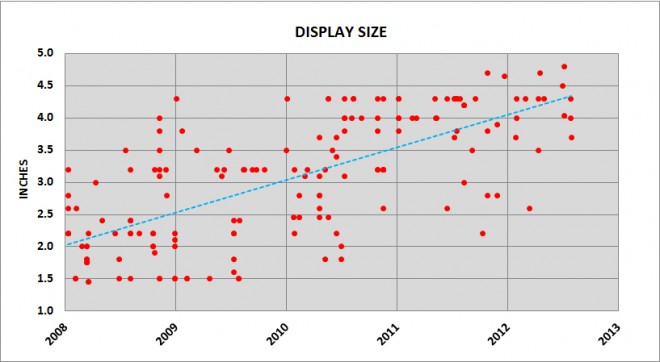
\includegraphics[width=110mm]{images/smartphoneSize2}
		\caption{Smartphone screens have been increasing ever since the iPhone launched in 2007.\cite{smartphoneSizeChart2}}
		\label{smartphoneSizeChart2}
	\end{figure}
	%http://www.pcworld.com/article/2455169/why-smartphone-screens-are-getting-bigger-specs-reveal-a-surprising-story.html

\hfill

%\url{https://developer.android.com/design/index.html}\\
%\url{https://developer.android.com/design/get-started/principles.html}
	\begin{figure}[ht!]
		\centering
		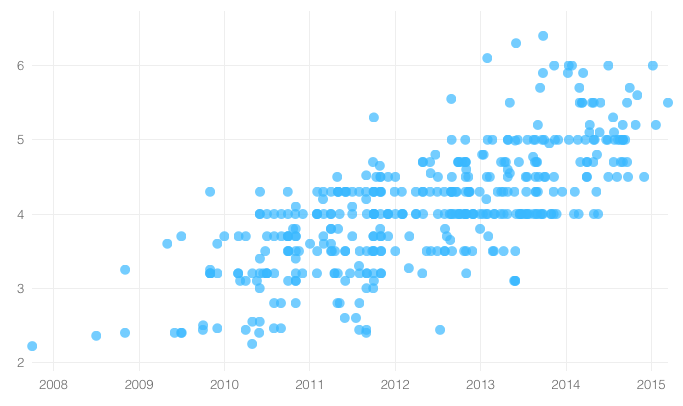
\includegraphics[width=110mm]{images/smartphoneSize}
		\caption{Smartphone screen sizes of the most popular of the currently available smartphones, where the x-axis shows the release date and the y-axis shows the screen size in inches.\cite{smartphoneSizeChart}}
		\label{smartphoneSizeChart}
	\end{figure}
	%http://www.pcworld.com/article/2455169/why-smartphone-screens-are-getting-bigger-specs-reveal-a-surprising-story.html

% Color schemes
% pre defined layouts
% pre defined typography (fonts)









\subsection{Limitations with Google Glass}
\label{subsec:limitations}
%Screen size
%Resolution
%Information on screen (possible result/discussion)
%How about people wearing glasses normally? Will the boss require employees to get lenses?
One early concern with Google Glass came from people who wore regular glasses every day, as Google Glass seemed to require separate frames. Isabelle Olsson at Google responded on the issue on April 12th 2012 with the following: ``We ideally want Project Glass to work for everyone, and we're experimenting with designs that are meant to be extendable to different types of frames.''~\cite{GoogleGlassFrameResponse}.

Today many eyecare providers have been trained for Google Glass and Glass frames. These trained eyecare providers are however mostly located in the United States~\cite{frameProviders}, but Google points out that many eyecare providers should be able to help replace the lenses on Google Glass' frames~\cite{framesGlass}.

% not relevant reference
%\url{http://www.google.com/glass/help/frames/} 
As described in an article posted on forbes in 2013~\cite{ackerman13}, a more alarming concern has been the health of the user's eyes. Concerns were raised regarding eye strain and misalignment of the user's eyes, as Google Glass placed a screen above one eye and not both. Google also saw these potential issues and approached Eli Peli, professor of ophthalmology who had been studying HMDs for two decades, as the development och Google Glass started.

Peli claimed that Google Glass has been designed with more safety and comfort in mind than previous, similar products. Peli pointed out that Google Glass is see-through and only covers a small part of the user's field of vision. As such Google Glass does not require a potentially poorly adjusted camera to capture the environment and display the environment to the user, which could cause eye strain.

Peli also pointed out that Google Glass is meant only to be used for short periods. Google Glass is meant to give the user notifications that can be quickly dealt with. The user should not be looking at the display for long periods of time, which would have the potential to lead to eye strain. While Peli stated that the risks are zero, he still claimed that the likelihood of Google Glass causing any damage is minimal.

%Eye pain? 
%\url{http://www.forbes.com/sites/eliseackerman/2013/03/04/could-google-glass-hurt-your-eyes-a-harvard-vision-scientist-and-project-glass-advisor-responds/}
%
%documented eye pain from looking at a screen for too long. Also conserns regarding looking at something that not both eyes can see. Can give headache and slighted eye aligntment.\\
%
Even though, according to Google's expert, there might not be any health risks involved, there is still a question of how much help Google Glass may be to users. A study performed in 2002~\cite{laramee02}, regarding the effects of OHMDs, showed that OHMDs may only be of help to users under controlled forms. Whenever the surrounding evnironment becomes too distracting, for instance within a moving crowd, performance decreases. The study however noted that pilots had been able to successfully turn HMD into a tool they could use to their advantage. Since the study was not carried out over a long period of time the participants were potentially not given enough time to get used to wearing and using their HMDs, explaining the poor performance when using a distracting background.

%HMD:s could potential be of great service to users as long as users take the time to get use to the HMD device.\cite{laramee02}\\

\subsection{Presenting Information on Google Glass}
\label{subsec:informationlimitedspace}
%The principles behind designing for glass is to keep the information relevant. Google ranks different computational devices and services in terms of time periods. Google talks about how the cloud stores information ``forever'', a computer keeps about a years worth of information, a mobile phone is keeping track of the last month and Glass are for the present.\\

%Therefore Google asks developers to keep the information relevant and simple. Glass is designed not to get in the way of the user and, as stated previously, be usable when the users wants to.\cite{glassDesignPrinciples}\\
%\url{https://developers.google.com/glass/design/principles}

	\begin{figure}[ht!]
		\centering
		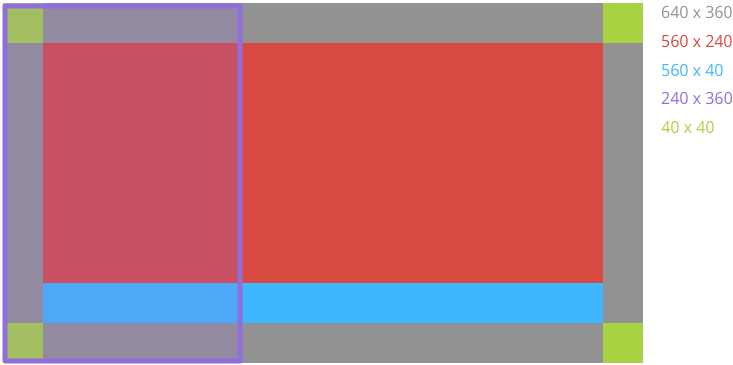
\includegraphics[width=110mm]{images/standard-template}
		\caption{Google provide developers with strict guidelines as to how they should use the limited space that Google Glass can present information on.\cite{glassDesignStyle}}
		\label{GlassDesignStyle}
	\end{figure}

%Google Glass is placed very close to the user's eye which makes the small projection seem Despite the fact that the display for Google Glass is placed very close to the user's eye the amount of information that can be displayed is still very limited. Google have therefore provided developers with a few guidelines when writing text which will be presented on Glass.\cite{glassDesignStyle} These guidelines, five in total,


% REWRITE !!!!
% \begin{itemize}
%	\item \textbf{Keep it brief.} Be concise, simple and precise. Look for alternatives to long text such as reading the content aloud, showing images or video, or removing features.
%	\item \textbf{Keep it simple.} Pretend you're speaking to someone who's smart and competent, but doesn't know technical jargon and may not speak English very well. Use short words, active verbs, and common nouns.
%	\item \textbf{Be friendly.} Use contractions. Talk directly to the reader using second person ("you"). If your text doesn't read the way you'd say it in casual conversation, it's probably not the way you should write it.
%	\item \textbf{Put the most important thing first.} The first two words (around 11 characters, including spaces) should include at least a taste of the most important information in the string. If they don't, start over. Describe only what's necessary, and no more. Don't try to explain subtle differences. They will be lost on most users.
%	\item \textbf{Avoid repetition.} If a significant term gets repeated within a screen or block of text, find a way to use it just once.
%\end{itemize}

%*** REWRITE !!!


\subsection{Similar Products}
\label{subsec:similarproducts}
Today there are several products, either already on the market or under development, that are more or less similar to Google Glass. The following is a short list (a more extensive list of devices can be found on Wikipedia~\cite{ohmdWiki}) describing some of the competition Google Glass faces, with each product shown in Figure ~\ref{imagesSimilarProducts}. 

	\begin{figure}[H]%ht!]
		\centering
    	\subfloat[Microsoft Hololens~\cite{hololens}]{{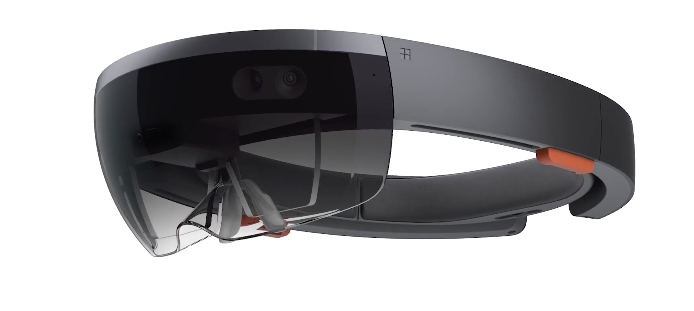
\includegraphics[width=70mm]{images/similarProducts/hololens}}}
    \qquad
    	\subfloat[Recon Jet~\cite{reconJet}]{{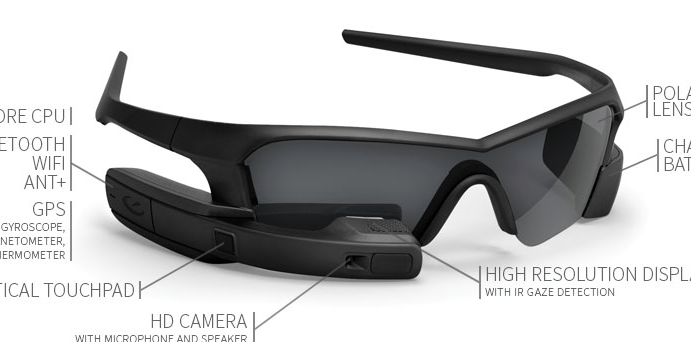
\includegraphics[width=70mm]{images/similarProducts/reconJet}}}
    \qquad
        \subfloat[GlassUp~\cite{glassUpFeatures}]{{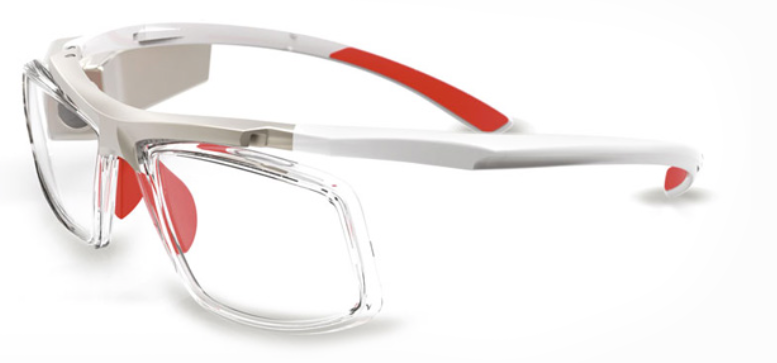
\includegraphics[width=70mm]{images/similarProducts/glassUp}}}
    \qquad
  	\subfloat[C Wear Interactive Glasses~\cite{pennyProducts}]{{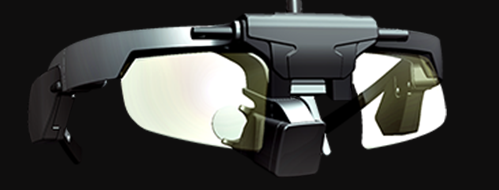
\includegraphics[width=70mm]{images/similarProducts/penny}}}
    \qquad
		\caption{There are many OHMD devices similar to Google Glass~\cite{ohmdWiki}.}
		\label{imagesSimilarProducts}
	\end{figure}
	

\subsubsection{Microsoft Hololens}

Microsoft's offer in the augmented reality device space is an HUD that displays information in front of both of the user's eyes. Microsoft's device is called Microsoft Hololens and can be seen in Figure~\ref{imagesSimilarProducts}~(a)~\cite{hololens}. 
%The intention, according to Microsoft, is not to be an immediate competitor to Google Glass. Microsoft's aim is not to make the same device as Google Glass. 
While Google Glass is meant to be worn at all times, Microsoft Hololens is rather a device users only wear when they intend to use Microsoft Hololens. Google Glass is, as Thad Starner stated~\cite{6504855}, meant to be an extension of the self and is meant to be worn at all times, even though the user might not be actively using Google Glass at the time, in order to bring helpful notifications and information to the user. Microsoft Hololens is rather a tool to be used actively for a certain purpose, such as modelling~\cite{hololensDemo}, and then put away. Google Glass may be used the same way if the user wants to, but that is not the intent.

The mot striking difference between Microsoft Hololens and Google Glass lies in the interaction with the real world. Google Glass is a two-dimensional (2D) display that sits slightly above the users line of sight% (see Section~\ref{subsec:googleglass})
. Microsoft Hololens, on the other hand, is meant to interact with the world even further.

Microsoft intends to give the user tools to work in a 3D space. Microsoft's concept video~\cite{hololensConceptVideo} of Microsoft Hololens shows examples of 3D modelling with the use of kinetic hand-movement detection. Microsoft Hololens will enable users to see what they are working on from different angles simply by walking around the object, just as if the object in question were real and had a physical mass.

\subsubsection{Recon Jet}

Recon Jet, seen in Figure~\ref{imagesSimilarProducts}~(b), is an HMD developed by Recon Instruments~\cite{reconJet}. Recon Jet is suited for athletes. Because of the target audience, Recon Jet has been fitted with a display that has high contrast in order to give good readability in high ambient lighting. The display's virtual image appears as  a 30 inch wide screen at approximately 2 meters distance~\cite{reconJetSpecs}, to be compared with Google Glass' virtual image which appears as a 25 inch high definition screen seen from a distance of 2.5 meters~\cite{GlassSpecs}.

Unlike Google Glass, Recon Jet's display is located below the user's line of sight, as seen in Figure~\ref{imagesSimilarProducts}. Recon Jet's target audience, athletes, are used to having their information below line of sight. For instance a bike may have dashboard mounted to the handlebar, or an athlete might be using a watch to check the time. Google Glass is meant to be worn at all times while the location and the brightness of the Recon Jet display indicates that Recon Jet, however, is meant to only be used while the athlete is working out and not more regularly.

\subsubsection{GlassUp}

GlassUp is an Italian company that received most of its founding for the HMD device, GlassUp~\cite{glassUp} (seen in Figure~\ref{imagesSimilarProducts}~(c)), through the crowd-funding site Indiegogo~\cite{glassUpIndiegogo}. GlassUp has been accused of being too similar to Google Glass, partially because of the name of the device~\cite{glassUpLegal}. GlassUp does however make distinctions between the two products. On GlassUp's Indiegogo page the company made the comparison that looking at Google Glass' display was similar to looking in the back view mirror while GlassUp was similar to looking out the windscreen. The comparison referenced the fact that Google Glass' display is located above the user's line of sight, similar to a rear view mirror.

GlassUp instead displays information close to the center of the user's line of sight. GlassUp claimed, on the company's Indiegogo page, that the display was placed closer to the center of the users line of sight so that there would be less strain on the user's eyes. However, the biggest difference from Google Glass is that GlassUp is meant only to act as a second screen. GlassUp is a ``receive only'' device which displays information from the device currently connected through bluetooth, for instance a smartphone. GlassUp does not do any calculations on its own and must stay connected to a bluetooth device in order to display information~\cite{glassUpIndiegogo}.

\subsubsection{C Wear Interactive Glasses}

C Wear Interactive Glasses~\cite{penny}, seen in Figure~\ref{imagesSimilarProducts}~(d), is an industry focused device developed by Penny in V{\"a}ster{\aa}s, Sweden~\cite{pennyCompany}. C Wear Interactive Glasses projects an image onto the actual glass in front of the user's right eye and as such covers a larger area than similar devices such as Google Glass, Recon Jet and GlassUp~\cite{pennyDisplay}. The display is said to be perceived as a 75 inch display at a distance of 2.1 meters~\cite{pennyProducts}. The projection is transparent which enables users to still see what is happening in front of them.

Being industry focused, C Wear Interactive Glasses is also equipped with a hands-free user interface  that does not require voice command. C Wear Interactive Glasses uses a jaw sensor which lies against the user's jawbone muscle. The sensor detects tension in the muscle, which registers as a click, to be compared with a touch on the Google Glass touchpad~\cite{pennyProducts}.

C Wear Interactive Glasses, similar to GlassUp, is designed to be connected to an external device~\cite{pennyProducts}. However, where GlassUp is connected through bluetooth C Wear Interactive Glasses is connected to the external device through an adapter which can send data and visual information via USB and HDMI. The external device can be a smartphone, a tablet, a PC or even a TV.
%\url{http://www.microsoft.com/microsoft-hololens/en-us}
%\url{http://www.searchenginejournal.com/google-glass-alternatives/67018/}
%\url{http://www.penny.se}

\subsection{Summary}
\label{subsec:summary}
%o   Introduce problem area / give relevant background info
%\\o   Introduction - Explain WHY you are doing this study
%\\o   Information - Background / your study in the wider context
%\\o   Similar work (projects, systems etc.)
%\\o   Summary - for this chapter
Google Glass was announced in 2012 along with the statement ``We think technology should work for you---to be there when you need it and get out of your way when you don't.''~\cite{GoogleGlassAnnouncement}. Google wanted to create a device where the user did not have to look down~\cite{tedtalkWhyGlass} as well as a device where the time between intention and action was minimised~\cite{6504855}. 

Google Glass (see Figure~\ref{GoogleGlassHardware}~(a) and~(b)) is an small HMD that is partially controlled with a touchpad mounted on the right hand side of the frames. The display sits slightly above the user's line of sight, on the right hand side. Google Glass' display is a projection that goes through an optic lense, creating a virtual image which makes the perception of the display to be equivalent of a 25 inch high definition screen seen from a distance of approximately 2.5 meters~\cite{GlassSpecs}.

Today there are many products similar to Google Glass either already on the market or in development. Microsoft Hololens is an HMD focused on letting the user work in a 3D space (with for instance 3D modelling~\cite{hololensDemo}) by covering both of the user's eyes. Recon Jet, GlassUp and C Wear Interactive Glasses are three products more similar to Google Glass in the sense that they only display information in front of one eye. However, Recon Jet is aimed at athletes, to be used while athletes are working out. GlassUp and C Wear Interactive Glasses are meant to be connected to an external device, such as a smartphone or a PC. Google Glass is a stand-alone device meant to be worn at all times.

The GUI of Google Glass is called a timeline and consists of a row of cards~\cite{ImagesGoogleGlassUI}. Cards are basic activities, such as a clock, but may also represent more in-depth applications, such as a game, on Google Glass called ``Immersions''. The center point of the timeline is the home screen and the first thing the user sees when turning on Google Glass. Cards to the left of the home screen are upcoming events, such as a flight, and cards to the right of the home screen are from the past, such as text messages. The user moves left on the timeline by swiping a finger backwards on the touchpad and in order to move right the user must swipe a finger forwards on the touchpad. 

In order to play sounds Google Glass uses a BCT which transfers sound through the bones of the skull~\cite{GlassSpecs}. The advantage of this technique is that external sound is not blocked out. In order to capture the environment Google Glass is also equipped with a 5 megapixles camera~\cite{GlassSpecs} and a microphone. Using the camera and the microphone the user may give input to Google Glass, for instance when using voice commands in order to control Google Glass hands-free.

The hands-free experience is also what sets Google Glass appart from regular smartphones. Smartphones must be held by the user or put on a table. The user must also look down at the screen of a smartphone, in contrast to Google Glass which puts the display slightly above the user's line of sight. Smartphones does however give the user a bit more control with multi-touch and touchscreen. Another advantage of smartphones is the larger screens. Smartphone screens have been increasing in size ever since the iPhone launched in 2007~\cite{smartphoneSizeChart2}. However, as HMDs increase in popularity, there is potential for a wider offering of models and screen sizes.

[TODO OVERGANG TILL QR KOD] The QR code was announced in 1994 by Denso Wave~\cite{qrCodeHistory}. The goal was to create a new form af barcode that could carry more information than a linear barcode and be easily read. While a conventional bardoce is capable of storing approximately 10 digits a QR code can store several thousand digits~\cite{qrCodeType}. A QR code also uses position fields which makes it readable from any direction, compared to a conventional barcode which can only be read horizontally~\cite{qrCodeAbout}. A QR code can be used to encode information, originally written with alphabetic characters, japanese symbols (Kanji) or numeric characters~\cite{qrCodeVersion}. 

information has been defined as ``a large number of examples from texts of different kinds''~\cite{informationDef1} and may be presented in a number of different ways. The four main ways of presenting information are text, images, sound and video. Text and images both have the advantage of being independent of time. Readers/viewers may perceive the information at their own pace. Images may also be divided into photographs and graphs. The difference of the two lies in the fact that graphs are used to present statistical information. Text and images does however both share the disadvantage of requiring readers/viewers vision.

Audio solves the problem of requiring the user's vision since audio uses a different sense. The listener may as a result multitask in terms of listening to the information being presented through audio while performing other tasks. For instance the listener may be listening to the radio while driving a car. In contrast to text and images audio is not independent of time.

Video shares the same disadvantage as audio in terms of not being independent of time. Video is, however, unique as video is the only form of presenting information which may combine images and show movement. Adding audio to video gives viewers the advantage of choice as they may choose to either watch or only listen.
[TODO SLUTKNORR PÅ KAPITLET]


%\subsection{Working handsfree}
%\label{subsec:workinghandsfree}
%Why?
%Multitasking (is this background or discussion?)
%Studies?
%\url{http://www.theguardian.com/science/2015/jan/18/modern-world-bad-for-brain-daniel-j-levitin-organized-mind-information-overload}
%\subsection{Multitasking on Google Glass}
%\label{subsec:multitaskingongoogleglass}







